%%%%%%%%%%%%%%%%%%%%%%%%%%%%%%% beamer %%%%%%%%%%%%%%%%%%%%%%%%%%%%%%%%%%%%%%%%%%%%%%%%%
% To run - pdflatex filename.tex
%      acroread filename.pdf
%%%%%%%%%%%%%%%%%%%%%%%%%%%%%%%%%%%%%%%%%%%%%%%%%%%%%%%%%%%%%%%%%%%%%%%%%%%%%%%%%%%%%%%%

\documentclass[compress,oilve]{beamer}
\mode<presentation>

\usetheme[]{CambridgeUS}
% other themes: AnnArbor, Antibes, Bergen, Berkeley, Berlin, Boadilla, boxes, CambridgeUS, Copenhagen, Darmstadt, default, Dresden, Frankfurt, Goettingen,
% Hannover, Ilmenau, JuanLesPins, Luebeck, Madrid, Maloe, Marburg, Montpellier, PaloAlto, Pittsburg, Rochester, Singapore, Szeged, classic

\usecolortheme{beaver}
% color themes: albatross, beaver, beetle, crane, default, dolphin,  fly, lily, orchid, rose, seagull, seahorse, sidebartab, whale, wolverine

\usefonttheme{professionalfonts}
% font themes: default, professionalfonts, serif, structurebold, structureitalicserif, structuresmallcapsserif


\hypersetup{pdfpagemode=FullScreen} % makes your presentation go automatically to full screen

% define your own colors:
\definecolor{Red}{rgb}{1,0,0}
\definecolor{Blue}{rgb}{0,0,1}
\definecolor{Green}{rgb}{0,1,0}
\definecolor{magenta}{rgb}{1,0,.6}
\definecolor{lightblue}{rgb}{0,.5,1}
\definecolor{lightpurple}{rgb}{0.8, 0.6, 0.9}
\definecolor{gold}{rgb}{.6,.5,0}
\definecolor{orange}{rgb}{1,0.4,0}
\definecolor{hotpink}{rgb}{1,0,0.5}
\definecolor{newcolor2}{rgb}{.5,.3,.5}
\definecolor{newcolor}{rgb}{0,.3,1}
\definecolor{newcolor3}{rgb}{1,0,.35}
\definecolor{darkgreen1}{rgb}{0, .35, 0}
\definecolor{darkgreen}{rgb}{0, .6, 0}
\definecolor{darkred}{rgb}{.75,0,0}
\definecolor{skyblue}{HTML}{75bbfd}

\definecolor{olive}{cmyk}{0.64,0,0.95,0.4}
\definecolor{purpleish}{cmyk}{0.75,0.75,0,0}

% can also choose different themes for the "inside" and "outside"

% \usepackage{beamerinnertheme_______}
% inner themes include circles, default, inmargin, rectangles, rounded

% \usepackage{beamerouterthemesmoothbars}
% outer themes include default, infolines, miniframes, shadow, sidebar, smoothbars, smoothtree, split, tree


\useoutertheme[subsection=true, height=40pt]{smoothbars}

% to have the same footer on all slides
%\setbeamertemplate{footline}[text line]{STUFF HERE!}
\setbeamertemplate{footline}[text line]{} % makes the footer EMPTY
% include packages
%

%show the page numbers in footnote
%\addtobeamertemplate{navigation symbols}{}{%
%	\usebeamerfont{footline}%
%	\usebeamercolor[fg]{footline}%
%	\hspace{1em}%
%	\insertframenumber/\inserttotalframenumber
%}

\setbeamercolor{footline}{fg=purpleish}
\setbeamerfont{footline}{series=\bfseries}

%add color to curent subsection
\setbeamertemplate{section in head/foot}{\hfill\tikz\node[rectangle, fill=darkred, rounded corners=1pt,inner sep=1pt,] {\textcolor{white}{\insertsectionhead}};}
\setbeamertemplate{section in head/foot shaded}{\textcolor{darkred}{\hfill\insertsectionhead}}

% Remove bullet of subsections
\setbeamertemplate{headline}
{%
	\begin{beamercolorbox}{section in head/foot}
		\insertsectionnavigationhorizontal{\textwidth}{}{}
	\end{beamercolorbox}%
}


% modify headlline, specially headline size
\setbeamertemplate{headline}{%
	\leavevmode%
	\hbox{%
		\begin{beamercolorbox}[wd=\paperwidth,ht=3.5ex,dp=1.125ex]{palette quaternary}%
			\insertsectionnavigationhorizontal{\paperwidth}{}{\hskip0pt plus1filll}
		\end{beamercolorbox}%
	}
}

\setbeamertemplate{footline}{%
	\leavevmode%
	\hbox{\begin{beamercolorbox}[wd=.5\paperwidth,ht=2.5ex,dp=1.125ex,leftskip=.3cm plus1fill,rightskip=.3cm]{author in head/foot}%
			\usebeamerfont{author in head/foot}\insertshortauthor ~ \insertshortinstitute
		\end{beamercolorbox}%
		\begin{beamercolorbox}[wd=.5\paperwidth,ht=2.5ex,dp=1.125ex,leftskip=.3cm,rightskip=.3cm plus1fil]{title in head/foot}%
			\usebeamerfont{title in head/foot}\insertshorttitle\hfill\insertframenumber\,/\,\inserttotalframenumber
	\end{beamercolorbox}}%
	\vskip0pt%
}


%\setbeamertemplate{navigation symbols}{}

\title{Generative Adversarial Networks (GANs)}
\author{ML Instruction Team, Fall 2022}
\institute[]{CE Department \newline  Sharif University of Technology \newline \newline}
\date[\today]{}
%\titlegraphic{\includegraphics[scale=.35]{example-image}}
\graphicspath{{figs/}}



%Write \usepackage{etex} just after the \documentclass line (it should be the first loaded package).
% \usepackage{etex}
\usepackage{subcaption}
\usepackage{multicol}
\usepackage{amsmath}
\usepackage{epsfig}
\usepackage{graphicx}
\usepackage[all,knot]{xy}
\xyoption{arc}
\usepackage{url}
\usepackage{multimedia}
\usepackage{hyperref}
\hypersetup{colorlinks,linkcolor=blue,citecolor=redorange,urlcolor=darkred}
\usepackage{multirow}
\usepackage[font={scriptsize}]{caption}
\usepackage{pgf}
\usepackage{fontspec}
%\setsansfont[Scale=MatchLowercase, BoldFont = * Bold, ItalicFont = * Italic]{Caladea}

%\usepackage{enumitem,xcolor}
%\newcommand{\labelitemi}{$\blacksquare$}
%\newcommand{\labelitemii}{$\diamond$}
%\newcommand{\labelitemiii}{$\square$}
%\newcommand{\labelitemiv}{$\ast$}
%\setbeamercolor*{item}{fg=red}


\usefonttheme{professionalfonts} 
\setbeamertemplate{itemize item}{\color{skyblue}$\blacksquare$}
\setbeamertemplate{itemize subitem}{\color{hotpink}$\blacktriangleright$}
\setbeamertemplate{itemize subsubitem}{\color{orange}$\bullet$}


\usepackage{anyfontsize}
\usepackage{t1enc}
\usepackage{tikz}
\usetikzlibrary{calc,trees,positioning,arrows,chains,shapes.geometric,decorations.pathreplacing,decorations.pathmorphing,shapes,matrix,shapes.symbols}



\newtheorem{proposition}[theorem]{Proposition}
\newtheorem{remark}[theorem]{Remark}
\newtheorem{assumption}[theorem]{Assumption}

\usepackage{fontspec,unicode-math}
\setmainfont{Consolas}[
    Scale=0.9,
    Path=./Fonts/,
    Extension = .ttf,
]
\setmonofont{Monaco}[
    Scale=0.9,
    Path=./Fonts/,
    Extension = .ttf,
]

\setsansfont[Scale=1]{Times New Roman}

%\usepackage{smartdiagram}
%\usesmartdiagramlibrary{additions}
%%%%%%%%%%%%%%%%%%%%%%%%%%%%%%%%%%%%%%%%%%%%%%%%%%%%%%%%%%%%%%%%%%%%%%%%%%%%%%%%%%%%%%%%%%%%
%%%%%%%%%%%%%%%%%%%%%%%%%%%%%% Title Page Info %%%%%%%%%%%%%%%%%%%%%%%%%%%%%%%%%%%%%%%%%%%
%%%%%%%%%%%%%%%%%%%%%%%%%%%%%%%%%%%%%%%%%%%%%%%%%%%%%%%%%%%%%%%%%%%%%%%%%%%%%%%%%%%%%%%%%%


%%%%%%%%%%%%%%%%%%%%%%%%%%%%%%%%%%%%%%%%%%%%%%%%%%%%%%%%%%%%%%%%%%%%%%%%%%%%%%%%%%%%%%%%%%
%%%%%%%%%%%%%%%%%%%%%%%%%%%%%% Begin Your Document %%%%%%%%%%%%%%%%%%%%%%%%%%%%%%%%%%%%%%%
%%%%%%%%%%%%%%%%%%%%%%%%%%%%%%%%%%%%%%%%%%%%%%%%%%%%%%%%%%%%%%%%%%%%%%%%%%%%%%%%%%%%%%%%%%
\begin{document}

%%%%%%%%%%%%%%%%%%%%%%%%%%%%%%%%%%%%%%%%%%%%%%%%%%%%%%%%%%%%%%%%%%%%%%%%%%%%%%%%%%%%%%%%%%
\fontsize{9}{9}
\begin{frame}[noframenumbering, plain]
	\titlepage
\end{frame}
\section{Introduction}

\frame{\frametitle{Discriminative vs Generative Models}

	\begin{itemize}
		\item Machine learning models can be classified into two types: Discriminative and Generative.
		\item A \alert{discriminative model} makes predictions on the unseen data based on conditional probability and can be used for classification or regression problems.
		\item A \alert{generative model} focuses on the latent distribution of a dataset to return a probability for an example.
		      \begin{figure}[htp]
			      \vspace{1ex}%
			      \centering
			      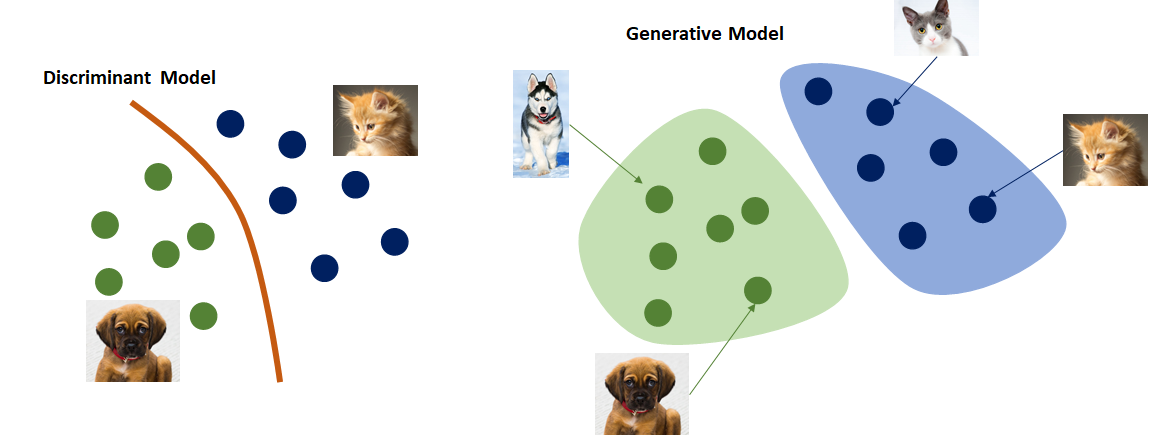
\includegraphics[width=10cm]{gen_disc}
			      \caption{Discriminative vs Generative Models \href{https://medium.com/@jordi299/about-generative-and-discriminative-models-d8958b67ad32}{Source}}
		      \end{figure}

	\end{itemize}
}


\frame{\frametitle{Generative Models}

	\begin{itemize}
		\item Generative models have two types:
		      \begin{itemize}
			      \item \alert{Explicit likelihood models} are defined by an explicit specification of the density, and so their unnormalized complete likelihood can be usually expressed in closed form.
			      \item \alert{Implicit probabilistic models} are defined naturally in a sampling procedure and often induce a likelihood function that cannot be expressed explicitly.
		      \end{itemize}
	\end{itemize}
	\begin{figure}
		\centering
		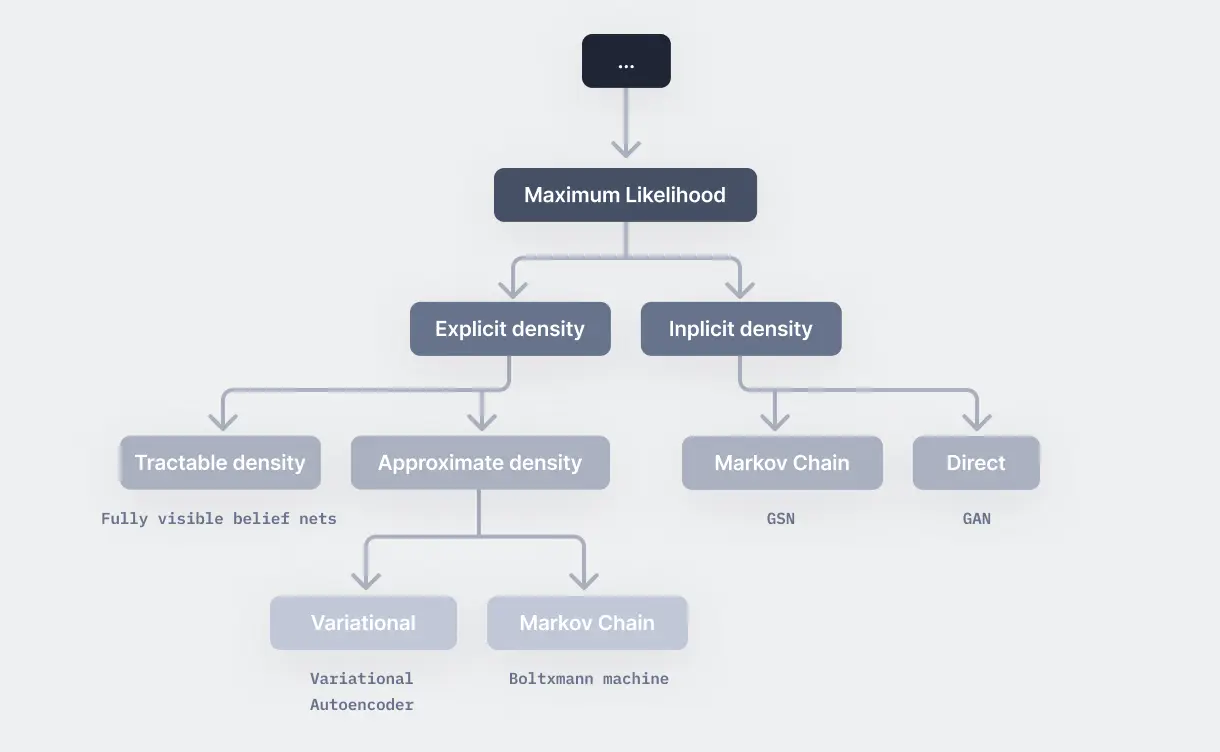
\includegraphics[width=6cm]{gen_models}
		\caption{IAN Goodfellow's presentation of Generative Models Taxonomy \href{https://arxiv.org/pdf/1701.00160.pdf}{Source}}
	\end{figure}
}

\frame{\frametitle{Generative Models}
	\begin{itemize}
		\item Generative models aim for a complete probabilistic description of the data. With these models, the goal is to construct the joint probability distribution $P(X, Y)$ – either directly or by first computing $P(X | Y)$ and $P(Y)$ – and then inferring the conditional probabilities required to classify new data.
		\item Generative models are used for:
		      \begin{enumerate}
			      \item \alert{Density estimation} is the task of estimating the probability density function (PDF) of a random variable.
			      \item \alert{Data generation} is the task of generating new data samples from a given distribution.
			      \item \alert{Data imputation} is the task of filling in missing data.
			      \item \alert{Data compression} is the task of reducing the amount of information required to represent a dataset.
		      \end{enumerate}
	\end{itemize}
}
\section{Architecture}

\frame{\frametitle{Generative Adversarial Networks - Architecture}
	\begin{itemize}
		\item So how do Generative Adversarial Networks work?
		\item GAN composes of two deep networks:
		      \begin{itemize}
			      \item The generator
			      \item The discriminator.
		      \end{itemize}
	\end{itemize}

	\hyperlink{gan}{
		\begin{figure}
			\centering
			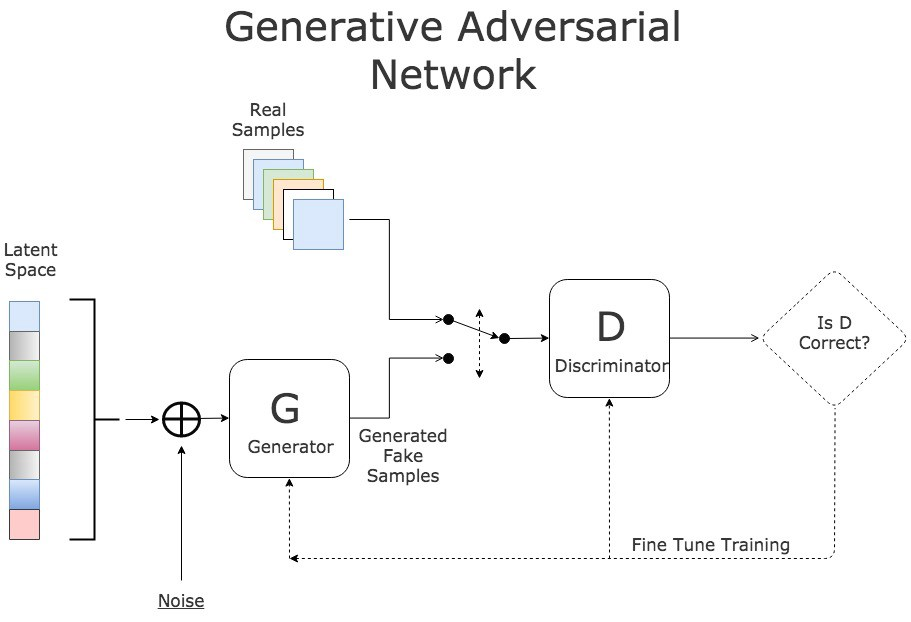
\includegraphics[width=7cm]{gan.jpeg}
		\end{figure}
	}
}

\frame{\frametitle{Generative Adversarial Networks - Structure}
	\hyperlink{gan_structure}{
		\begin{figure}
			\centering
			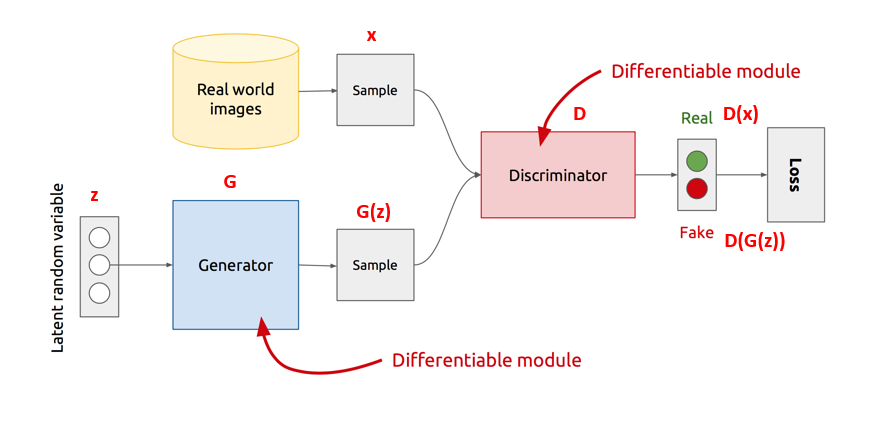
\includegraphics[width=6cm]{../images/GAN_Structure.png}
		\end{figure}
	}

	\begin{itemize}
		\item So let's look at the full picture
		\item Let $G_\phi$ be the generator and $D_\theta$ be the discriminator ($\phi$ and $\theta$ are the parameters of $G$ and $D$, respectively)
		\item We have a neural network based generator which takes as input a noise vector $z \sim N(0, I)$ and produces $G_\phi(z) = X$
		\item We have a neural network based discriminator which could take as input a real $X$ or a generated $X = G_\phi(z)$ and classify the input as real/fake
	\end{itemize}
}


\frame{\frametitle{GAN: Loss Function}
	\begin{center}
		\tikzstyle{hidden_neuron}=[circle,draw=blue!50,fill=cyan!10,thick,minimum size=4mm]
\begin{tikzpicture}
\newcommand*{\xpos}{10}
\newcommand*{\ypos}{10}
\newcommand*{\rectstarty}{6}
\newcommand*{\rectendy}{6.5}


%%%%%%%%%%%%%%Generator

% Generator
{
	\renewcommand*{\xpos}{20}
	\draw[rounded corners,fill=green!12] (\xpos-0.5, \rectstarty+1) rectangle (\xpos+2, \rectendy+1) {};
	\node (N) at (\xpos+0.75,\rectendy+0.75) {\small{Generator}};

	% Sample z
	\draw[rounded corners,fill=cyan!20] (\xpos-0.5, \rectstarty) rectangle (\xpos+2, \rectendy) {};
	\node[hidden_neuron] (N1) at (\xpos,\rectstarty+0.25) {};
	\node[hidden_neuron] (N2) at (\xpos+1*0.5,\rectstarty+0.25) {};
	\node[hidden_neuron] (N3) at (\xpos+2*0.5,\rectstarty+0.25) {};
	\node[hidden_neuron] (N4) at (\xpos+3*0.5,\rectstarty+0.25) {};
	\node (N) at (\xpos+1,\rectstarty-0.5) {\small{$z \sim N(0,I)$}};

	% Bottom arrow
	\draw[->,thick,black] (\xpos+0.75,\rectendy) -- (\xpos+0.75,\rectendy+0.5);

	% Images
	\node (N) at (\xpos+0.75,\rectstarty+2.2) {
\includegraphics[scale=0.1]{images/two_gen.png}};

	% Top arrow
	\draw[->,thick,black] (\xpos+0.75,\rectendy+1) -- (\xpos+0.75,\rectendy+1.5);
}
%%%%%%%%%%%%%%%Real world images
{
	\renewcommand*{\xpos}{23}

	% Real Images
	\draw[rounded corners,fill=green!12] (\xpos-0.5, \rectstarty+1) rectangle (\xpos+2, \rectendy+1) {};
	\node (N) at (\xpos+0.75,\rectendy+0.75) {\small{Real Images}};

	% Images
	\node (N) at (\xpos+0.75,\rectstarty+2.2) {
\includegraphics[scale=0.1]{images/two_real.png}};

	% Top arrow
	\draw[->,thick,black] (\xpos+0.75,\rectendy+1) -- (\xpos+0.75,\rectendy+1.5);

	\renewcommand*{\xpos}{23}
	\draw[->,thick,black] (\xpos+0.75,\rectendy+1.9) -- (\xpos+0.75-0.7,\rectstarty+3);
}
%%%%%%%%%%%%%%%% Discriminator
{
	\renewcommand*{\xpos}{21.5}
	% Discriminator
	\draw[rounded corners,fill=green!12] (\xpos-0.5, \rectstarty+3) rectangle (\xpos+2, \rectendy+3) {};
	\node (N) at (\xpos+0.75,\rectendy+2.75) {\small{Discriminator	}};
	{
		\draw[->,thick,black] (\xpos+0.75,\rectendy+3) -- (\xpos+0.75,\rectendy+3.4);
		\node (N) at (\xpos+0.75,\rectendy+3.52) {\small {Real or Fake}};
	}

	% Arrows
	\renewcommand*{\xpos}{20}
	\draw[->,thick,black] (\xpos+0.75,\rectendy+1.9) -- (\xpos+0.75+0.7,\rectstarty+3);
}
\end{tikzpicture}
	\end{center}

	\begin{itemize}
		\item What should be the objective function of the overall network?
		\item Let's look at the objective function of the generator first
		\item Given an image generated by the generator as $G_\phi(z)$ the discriminator assigns a score $D_\theta(G_\phi(z))$ to it
		\item This score will be between $0$ and $1$ and will tell us the probability of the image being real or fake
	\end{itemize}
}

\frame{\frametitle{GAN: Loss Function}
	\vspace*{-1cm}
	\begin{itemize}
		\item For a given $z$, the generator would want to maximize  $\log D_\theta(G_\phi(z))$ (log likelihood) or minimize $\log (1 - D_\theta(G_\phi(z)))$
		\item This is just for a single $z$ and the generator would like to do this for all possible values of $z$,
		\item For example, if $z$ was discrete and drawn from a uniform distribution (\textit{i.e.}, $p(z) = \frac{1}{N} ~ \forall z$) then the generator's objective function would be
		      $$ \min\limits_{\phi}  \sum_{i=1}^{N} \frac{1}{N} \log (1 - D_{\theta}(G_{\phi}(z))) $$
	\end{itemize}
}

\frame{\frametitle{GAN: Loss Function}
	\begin{itemize}
		\item However, in our case, z is continuous and not uniform ($z \sim N(0, I)$) so the equivalent objective function would be
		      $$\min \limits_{\phi} \int p(z) \log(1 - D_{\theta}(G_{\phi}(z)))$$
		      $$\min \limits_{\phi}  E_{_{z \sim p(z)}} [\log (1 - D_{\theta}(G_{\phi}(z)))] $$
	\end{itemize}

	\hyperlink{Binglin}{
		\begin{figure}
			\centering
			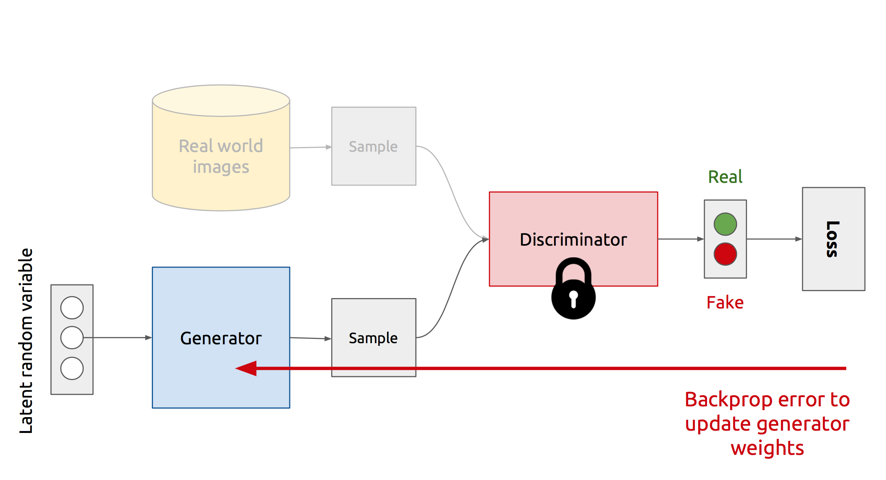
\includegraphics[width=8cm]{../images/Gen.png}
		\end{figure}
	}
}

\frame{\frametitle{GAN: Loss Function}
	\hyperlink{Binglin}{
		\begin{figure}
			\centering
			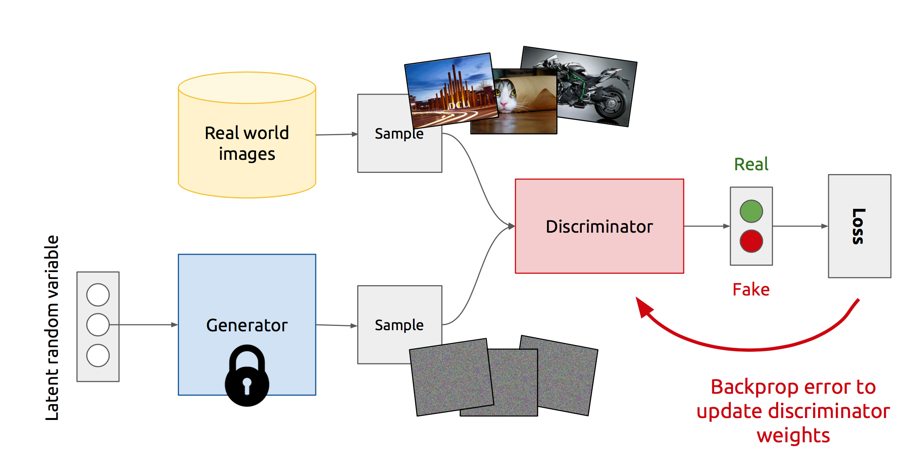
\includegraphics[width=8cm]{../images/Disc.png}
		\end{figure}
	}
	\begin{itemize}
		\item Now let's look at the discriminator
		\item The task of the discriminator is to assign a high score to real images and a low score to fake images
		\item And it should do this for all possible real images and all possible fake images
		\item In other words, it should try to maximize the following objective function
		      $$ \max_{\theta} E_{_{x \sim p_{data}}} [\log D_{\theta}(x)]
			      \newline + E_{_{z \sim p(z)}} [\log (1 - D_{\theta}(G_{\phi}(z)))] $$
	\end{itemize}
}

\frame{\frametitle{GAN: Loss Function}
	\vspace*{-1cm}
	\begin{itemize}
		\item If we put the objectives of the generator and discriminator together we get a minimax game
		      \begin{align*}
			      \min\limits_{\phi}\hspace*{2mm} \max\limits_{\theta} \hspace*{4mm} [ & \mathbb{E}_{x \sim p_{data}} \log D_{\theta}(x)                   \\
			                                                                           & ~~~+ \mathbb{E}_{z \sim p(z)} \log(1- D_{\theta}(G_{\phi}(z)) ) ]
		      \end{align*}
		\item The first term in the objective is only w.r.t. the parameters of the discriminator ($\theta$)

		\item The second term in the objective is w.r.t. the parameters of the generator ($\phi$) as well as the discriminator ($\theta$)
		\item The discriminator wants to maximize the second term whereas the generator wants to minimize it (hence it is a two-player game)
	\end{itemize}
}
\section{Training}

\begin{frame}
	\frametitle{GAN - Training}
	\begin{itemize}
		\item So the overall training proceeds by alternating between these two step

		\item \textbf{Step 1:} Gradient Ascent on Discriminator
		      $$ \max\limits_{\theta}\hspace*{2mm} [\mathbb{E}_{x \sim p_{data}} \log D_{\theta}(x)
			      \newline
			      + \mathbb{E}_{z \sim p(z)} \log(1- D_{\theta}(G_{\phi}(z)) ) ]$$

		\item \textbf{Step 2:} Gradient Descent on Generator
		      $$   \min\limits_{\phi}\hspace*{2mm} \mathbb{E}_{z \sim p(z)} \log(1- D_{\theta}(G_{\phi}(z)) )$$

		\item In practice, the above generator objective does not work well and we use a slightly modified objective
		\item Let us see why
	\end{itemize}
\end{frame}

\frame{\frametitle{GAN - Training}
	\begin{center}
		\hyperlink{miteshk}{
			\begin{figure}
				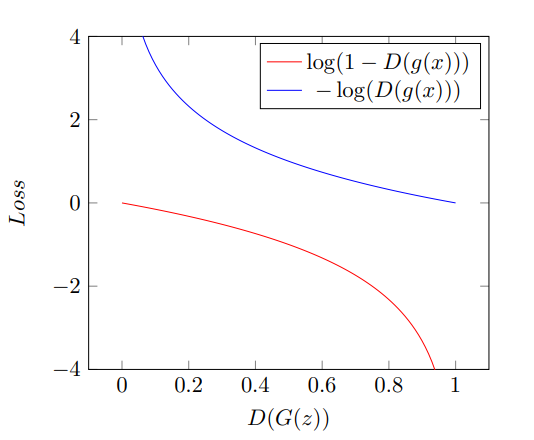
\includegraphics[width=5cm]{images/chart.png}
			\end{figure}
		}
	\end{center}
	\begin{itemize}
		\item When the sample is likely fake, we want to give a feedback to the generator (using gradients)
		\item However, in this region where $D(G(z))$ is close to 0, the curve of the loss function is very flat and the gradient would be close to $0$
		\item Trick: Instead of minimizing the likelihood of the discriminator being correct, maximize the likelihood of the discriminator being wrong
		\item In effect, the objective remains the same but the gradient signal becomes better
	\end{itemize}
}

\section{Architecture}
\begin{frame}
    \frame{\frametitle{Generative Adversarial Networks - Architecture}}
	% \myheading{Module 23.2: Generative Adversarial Networks - Architecture}
\end{frame}

\begin{frame}
	\begin{itemize}
		\item<1-> We will now look at one of the popular neural networks used for the generator and discriminator (Deep Convolutional GANs)
		For discriminator, any CNN based classifier with 1 class (real) at the output can be used (e.g. VGG, ResNet, etc.)
	\end{itemize}
	\visible<1->{
		\begin{center}
		\begin{figure}
          \hyperlink{DCGAN}{
			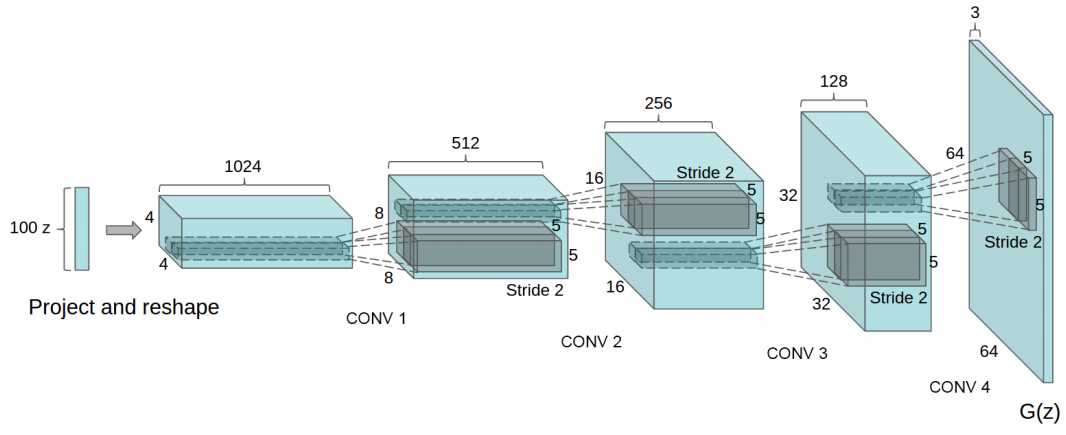
\includegraphics[scale=0.21]{images/dcgan_gen.png}
			\caption{Generator (Redford et al 2015) (left) and discriminator (Yeh et al 2016) (right) used in DCGAN}
          }
		\end{figure}
		\end{center}
	}
\end{frame}

\begin{frame}
	Architecture guidelines for stable Deep Convolutional GANs
	\begin{itemize}
		\item Replace any pooling layers with strided convolutions (discriminator) and fractional-strided convolutions (generator).
		\item Use batchnorm in both the generator and the discriminator.
		\item Remove fully connected hidden layers for deeper architectures.
		\item Use ReLU activation in generator for all layers except for the output, which uses tanh.
		\item Use LeakyReLU activation in the discriminator for all layers
	\end{itemize}
    \hyperlink{miteshk}{
        \begin{figure}
            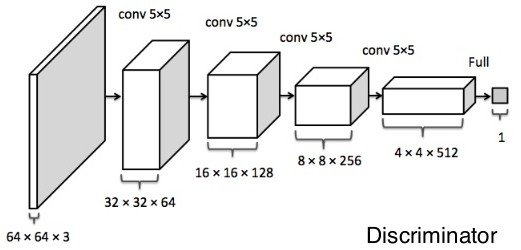
\includegraphics[scale=0.32]{images/dcgan_disc.jpg}
            \caption{Generator (Redford et al 2015) (left) and discriminator (Yeh et al 2016) (right) used in DCGAN}
        \end{figure}\
    }
\end{frame}


\begin{frame}
	\frame{\frametitle{Deep Convolutional GANs}}
	% \myheading{Module 23.2: Generative Adversarial Networks - Architecture}
\end{frame}

\begin{frame}
	\begin{itemize}
		\item<1-> We will now look at one of the popular neural networks used for the generator and discriminator (Deep Convolutional GANs)
			For discriminator, any CNN based classifier with 1 class (real) at the output can be used (e.g. VGG, ResNet, etc.)
	\end{itemize}
	\visible<1->{
		\begin{center}
			\begin{figure}
				\hyperlink{DCGAN}{
					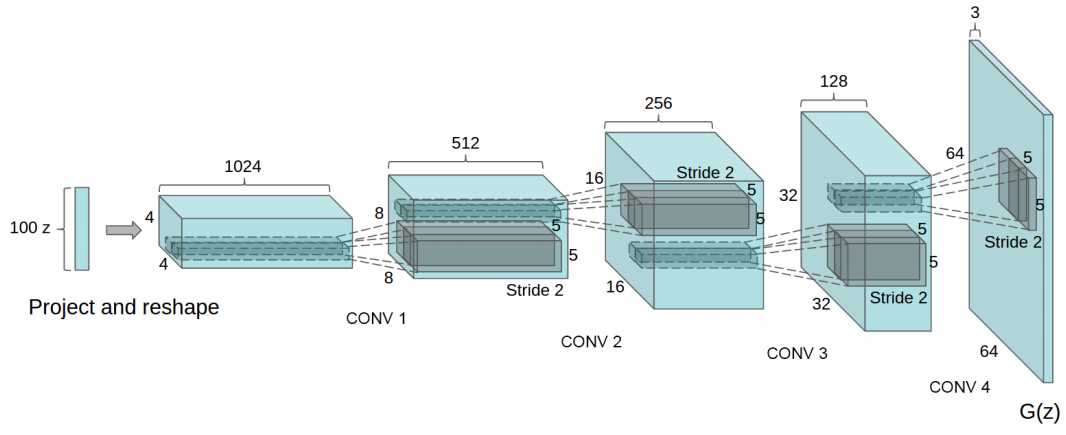
\includegraphics[scale=0.21]{images/dcgan_gen.png}
					\caption{Generator (Redford et al 2015) (left) and discriminator (Yeh et al 2016) (right) used in DCGAN}
				}
			\end{figure}
		\end{center}
	}
\end{frame}

\begin{frame}
	Architecture guidelines for stable Deep Convolutional GANs
	\begin{itemize}
		\item Replace any pooling layers with strided convolutions (discriminator) and fractional-strided convolutions (generator).
		\item Use batchnorm in both the generator and the discriminator.
		\item Remove fully connected hidden layers for deeper architectures.
		\item Use ReLU activation in generator for all layers except for the output, which uses tanh.
		\item Use LeakyReLU activation in the discriminator for all layers
	\end{itemize}
	\hyperlink{miteshk}{
		\begin{figure}
			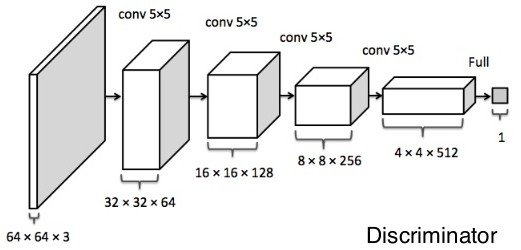
\includegraphics[scale=0.32]{images/dcgan_disc.jpg}
			\caption{Generator (Redford et al 2015) (left) and discriminator (Yeh et al 2016) (right) used in DCGAN}
		\end{figure}\
	}
\end{frame}


% \section{The Math Behind it}
\begin{frame}
    \frame{\frametitle{Generative Adversarial Networks - The Math Behind it}}
	% \myheading{Module 23.3: Generative Adversarial Networks - The Math Behind it}
\end{frame}

\begin{frame}
	\begin{itemize}
		\item<1-> We will now delve a bit deeper into the objective function used by GANs and see what it implies
		\item<2-> Suppose we denote the true data distribution by $p_{data}(x)$ and the distribution of the data generated by the model as $p_G(x)$
		\item<3-> What do we wish should happen at the end of training? 
					\visible<4->{ $$p_G(x) = p_{data}(x)$$ }
		\item<5-> Can we prove this formally even though the model is not explicitly computing this density?
		\item<6-> We will try to prove this over the next few slides
	\end{itemize}
\end{frame}

\begin{frame}
	\begin{block}{Theorem}
		The global minimum of the virtual training criterion $C(G)=\underset{D}{max} ~V(G,D)$ is achieved \textbf{if and only if} $p_G=p_{data}$\\
	\end{block}

	\begin{center}
		\visible<2->{\textbf{is equivalent to}}
	\end{center}

	\visible<3->
	{
		\begin{block}{Theorem}
			\begin{enumerate}
				\item \textbf{If} $p_G=p_{data}$ then the global minimum of the virtual training criterion $C(G)=\underset{D}{max} ~V(G,D)$ is achieved  \textbf{and}
				\item<4-> The global minimum of the virtual training criterion $C(G)=\underset{D}{max} ~V(G,D)$ is achieved \textbf{only if} $p_G=p_{data}$
			\end{enumerate}
		\end{block}
	}
	% \textbf{To Prove:}
	% \begin{itemize}[<+->]
	% 	\item The global minimum of the virtual training criterion $C(G)=\underset{D}{max} ~V(G,D)$ is achieved if and only if $p_G=p_{data}$
	% 	\item Any theorem containing an ``if and only if" condition can be split into two parts:
	% 	\begin{itemize}[<+->]
	% 		\item If $p_G=p_{data}$ then the global minimum of the virtual training criterion $C(G)=\underset{D}{max} ~V(G,D)$ is achieved
	% 		\item If the global minimum of the virtual training criterion $C(G)=\underset{D}{max} ~V(G,D)$ is achieved then $p_G=p_{data}$
	% 	\end{itemize}
	% \end{itemize}
\end{frame}

\begin{frame}
	\begin{block}{Outline of the Proof}
	\textbf{The `if' part:} The global minimum of the virtual training criterion $C(G)=\underset{D}{max} ~V(G,D)$ is achieved \textbf{if} $p_G=p_{data}$
		\begin{enumerate}
			\item[(a)]<2-> \alert<6>{Find the value of $V(D,G)$ when the generator is optimal \textit{i.e.}, when $p_G=p_{data}$}
			\item[(b)]<3-> Find the value of $V(D,G)$ for other values of the generator \textit{i.e.}, for any $p_G$ such that $p_G \neq p_{data}$
			\item[(c)]<4-> Show that $a < b$ $\forall$ $p_G \neq p_{data}$(and hence the minimum $V(D,G)$ is achieved when $p_G=p_{data}$)
		\end{enumerate}
	\vspace{5mm}
	\textbf{The `only if' part:} The global minimum of the virtual training criterion $C(G)=\underset{D}{max} ~V(G,D)$ is achieved \textbf{only if} $p_G=p_{data}$
	\begin{itemize}
		\item<5-> Show that when $V(D,G)$ is minimum then $p_G=p_{data}$
	\end{itemize}
	\end{block}
\end{frame}

\begin{frame}
	\begin{itemize}[<+->]
		\item First let us look at the objective function again 
				$$ \min\limits_{\phi}~ \max\limits_{\theta} \hspace*{4mm} [\mathbb{E}_{x \sim p_{data}} \log D_{\theta}(x) + \mathbb{E}_{z \sim p(z)} \log(1- D_{\theta}(G_{\phi}(z)) ) ] $$

		\item We will expand it to its integral form
			$$\min\limits_{\phi}~ \max\limits_{\theta} ~  \int_x p_{data}(x) \log D_{\theta}(x) + \int_z p(z) \log(1 - D_{\theta}(G_{\phi}(z)))$$
		\item Let $p_G(X)$ denote the distribution of the $X$'s generated by the generator and since $X$ is a function of $z$ we can replace the second integral as shown below
			$$\min\limits_{\phi}~ \max\limits_{\theta} ~  \int_x p_{data}(x) \log D_{\theta}(x) + \int_x p_G(x) \log(1 - D_{\theta}(x))$$
		% <replace the second interval involving z by x>
		\item The above replacement follows from the \textit{law of the unconscious statistician} \href{https://en.wikipedia.org/wiki/Law_of_the_unconscious_statistician}{(click to link of wikipedia page)}
	\end{itemize}
\end{frame}

\begin{frame}[shrink=10]
	\begin{itemize}[<+->]
		\item Okay, so our revised objective is given by
			$$\min\limits_{\phi}~ \max\limits_{\theta} ~ \int_x \left(p_{data}(x) \log D_{\theta}(x) +  p_G(x) \log(1 - D_{\theta}(x))\right)dx$$
		\item Given a generator G, we are interested in finding the optimum discriminator D which will maximize the above objective function
		\item The above objective will be maximized when the quantity inside the integral is maximized $\forall x$
		\item To find the optima we will take the derivative of the term inside the integral w.r.t. $D$ and set it to zero
			\begin{align*}
				\visible<5->{\frac{d}{d(D_\theta(x))}\left(p_{data}(x) \log D_{\theta}(x) +  p_{G}(x) \log(1 - D_{\theta}(x))\right) &= 0\\}
				\visible<6->{p_{data}(x) \frac{1}{D_{\theta}(x)} + p_{G}(x) \frac{1}{1-D_{\theta}(x)}(-1) &= 0\\}
				\visible<7->{\frac{p_{data}(x)}{D_{\theta}(x)} &=  \frac{p_{G}(x)}{1-D_{\theta}(x)} \\}
				\visible<8->{(p_{data}(x))(1-D_{\theta}(x)) &=  (p_{G}(x))(D_{\theta}(x)) \\}
				\visible<9->{D_\theta(x) &= \frac{p_{data}(x)}{p_{G}(x) + p_{data}(x)}}
			\end{align*}
		% <show the steps of the derivation ending with $D_\theta(x) = \frac{p_{data}}{p_{data} + p_{data}}$
	\end{itemize}
\end{frame}

\begin{frame}
	\begin{itemize}[<+->]
		\item This means for any given generator 
			$$D^{*}_G({G}(x)) = \frac{p_{data}(x)}{p_{data}(x) + p_G(x)}$$
		\item Now the if part of the theorem says ``if $p_G=p_{data}$ ...."
		\item So let us substitute $p_G = p_{data}$ into  $D^{*}_G({G}(x))$ and see what happens to the loss functions
		\begin{align*}
			\visible<4->{D^{*}_{{G}} &= \frac{p_{data}}{p_{data} + p_G} = \frac{1}{2}\\}
			\visible<5->{V({{G}},D^*_{{G}}) &= \int_x p_{data}(x) \log D(x) + p_G(x) \log\left(1-D(x)\right) dx\\  }
			\visible<6->{&= \int_x p_{data}(x) \log \frac{1}{2} + p_G(x) \log\left(1-\frac{1}{2}\right) dx\\}
			\visible<7->{&=  \log 2 \int_x p_G(x)dx - \log 2 \int_x p_{data}(x)dx		\\}
			\visible<8->{&= -2 \log 2 ~~~~~= -\log 4}
				    % &= <some trickery> see steps here https://srome.github.io/An-Annotated-Proof-of-Generative-Adversarial-Networks-with-Implementation-Notes\\
		\end{align*}
	\end{itemize}
\end{frame}

\begin{frame}
	\begin{block}{Outline of the Proof}
	\textbf{The `if' part:} The global minimum of the virtual training criterion $C(G)=\underset{D}{max} ~V(G,D)$ is achieved \textbf{if} $p_G=p_{data}$
		\begin{enumerate}
			\item[(a)] \color{gray}{Find the value of $V(D,G)$ when the generator is optimal \textit{i.e.}, when $p_G=p_{data}$} \color{black}
			\item[(b)] \alert<2>{Find the value of $V(D,G)$ for other values of the generator \textit{i.e.}, for any $p_G$ such that $p_G \neq p_{data}$}
			\item[(c)] Show that $a < b$ $\forall$ $p_G \neq p_{data}$(and hence the minimum $V(D,G)$ is achieved when $p_G=p_{data}$)
		\end{enumerate}
	\vspace{5mm}
	\textbf{The `only if' part:} The global minimum of the virtual training criterion $C(G)=\underset{D}{max} ~V(G,D)$ is achieved \textbf{only if} $p_G=p_{data}$
	\begin{itemize}
		\item Show that when $V(D,G)$ is minimum then $p_G=p_{data}$
	\end{itemize}
	\end{block}
\end{frame}

\begin{frame}
	\begin{itemize}[<+->]
		\item So what we have proved so far is that if the generator is optimal ($p_G = p_{data}$) the discriminator's loss value is $-\log 4$
		\item We still haven't proved that this is the minima
		\item For example, it is possible that for some $p_G \neq p_{data}$, the discriminator's loss value is lower than $-\log 4$
		\item To show that the discriminator achieves its lowest value ``if $p_G = p_{data}$", we need to show that for all other values of $p_G$ the discriminator's loss value is greater than $-\log 4$
	\end{itemize}
\end{frame}

\begin{frame}[shrink=25]
	\begin{itemize}[<+->]
		\item \scalebox{1.5}{To show this we will get rid of the assumption that $p_G=p_{data}$}
		% \item The entire derivation from the blog upto
		% $C(G)=-log4+KL(pdata||pdata+pG2)+KL(pG||pdata+pG2)$
	\end{itemize}
	\begin{align*}
		\visible<2->{C(G) &= \int_x \left[p_{data}(x) \log\left(\frac{p_{data}(x)}{p_G(x)+p_{data}(x)}\right) + p_G(x) \log\left(1-\frac{p_{data}(x)}{p_G(x)+p_{data}(x)}\right)\right]dx\\}
			\visible<3->{&= \int_x \left[p_{data}(x) \log\left(\frac{p_{data}(x)}{p_G(x)+p_{data}(x)}\right) + p_G(x) \log\left(\frac{p_G(x)}{p_G(x)+p_{data}(x)}\right) + (\log2-\log2)(p_{data}+p_{G})\right]dx\\}
			\visible<4->{&= -\log2 \int_x \left(p_G(x) + p_{data}(x)\right)dx \\
			&~~~~~+ \int_x \left[p_{data}(x) \left(\log 2+\log\left(\frac{p_{data}(x)}{p_G(x)+p_{data}(x)}\right)\right) 
					+ p_G(x)\left(\log2 + \log\left(\frac{p_G(x)}{P{p_G(x)+p_{data}(x)}}\right)\right)\right]dx \\}
			\visible<5->{&= -\log2 (1+1) \\
			&~~~~~+ \int_x \left[p_{data}(x) \log\left(\frac{p_{data}(x)}{\frac{p_G(x)+p_{data}(x)}{2}}\right) 
					+ p_G(x)\log\left(\frac{p_{G}(x)}{\frac{p_G(x)+p_{data}(x)}{2}}\right)\right]dx \\}
			\visible<6->{&= -\log4 + KL\left(p_{data}\|\frac{p_G(x)+p_{data}(x)}{2}\right) + KL\left(p_G\|\frac{p_G(x)+p_{data}(x)}{2}\right)}
	\end{align*}
\end{frame}

\begin{frame}
	\begin{block}{Outline of the Proof}
	\textbf{The `if' part:} The global minimum of the virtual training criterion $C(G)=\underset{D}{max} ~V(G,D)$ is achieved \textbf{if} $p_G=p_{data}$
		\begin{enumerate}
			\item[(a)] \color{gray}{Find the value of $V(D,G)$ when the generator is optimal \textit{i.e.}, when $p_G=p_{data}$} \color{black}
			\item[(b)] \color{gray}{Find the value of $V(D,G)$ for other values of the generator \textit{i.e.}, for any $p_G$ such that $p_G \neq p_{data}$} \color{black}
			\item[(c)] \alert<2>{Show that $a < b$ $\forall$ $p_G \neq p_{data}$(and hence the minimum $V(D,G)$ is achieved when $p_G=p_{data}$)}
		\end{enumerate}
	\vspace{5mm}
	\textbf{The `only if' part:} The global minimum of the virtual training criterion $C(G)=\underset{D}{max} ~V(G,D)$ is achieved \textbf{only if} $p_G=p_{data}$
	\begin{itemize}
		\item Show that when $V(D,G)$ is minimum then $p_G=p_{data}$
	\end{itemize}
	\end{block}
\end{frame}

\begin{frame}
	\begin{itemize}[<+->]
		\item Okay, so we have 
			$$C(G)=-\log 4 + KL\left(p_{data}||\frac{p_{data}+p_{g}}{2}\right)+KL\left(p_G||\frac{p_{data}+p_G}{2}\right)$$
		\item We know that KL divergence is always $\geq 0$
			$$\therefore C(G) \geq -\log 4$$
		\item Hence the minimum possible value of $C(G)$ is $-\log 4$ 
		\item But this is the value that $C(G)$ achieves when $p_G = p_{data}$ (and this is exactly what we wanted to prove)
		\item We have, thus, proved the \textbf{if part} of the theorem
	\end{itemize}
\end{frame}

\begin{frame}
	\begin{block}{Outline of the Proof}
	\textbf{The `if' part:} The global minimum of the virtual training criterion $C(G)=\underset{D}{max} ~V(G,D)$ is achieved \textbf{if} $p_G=p_{data}$
		\begin{enumerate}
			\item[(a)] \color{gray}{Find the value of $V(D,G)$ when the generator is optimal \textit{i.e.}, when $p_G=p_{data}$} \color{black}
			\item[(b)] \color{gray}{Find the value of $V(D,G)$ for other values of the generator \textit{i.e.}, for any $p_G$ such that $p_G \neq p_{data}$} \color{black}
			\item[(c)] \color{gray}{Show that $a < b$ $\forall$ $p_G \neq p_{data}$(and hence the minimum $V(D,G)$ is achieved when $p_G=p_{data}$)} \color{black}
		\end{enumerate}
	\vspace{5mm}
	\textbf{The `only if' part:} The global minimum of the virtual training criterion $C(G)=\underset{D}{max} ~V(G,D)$ is achieved \textbf{only if} $p_G=p_{data}$
	\begin{itemize}
		\item \alert<2>{Show that when $V(D,G)$ is minimum then $p_G=p_{data}$}
	\end{itemize}
	\end{block}
\end{frame}

\begin{frame}[shrink=15]
	\begin{itemize}[<+->]
		\item Now let's look at the other part of the theorem\\
			If the global minimum of the virtual training criterion $C(G)=\underset{D}{max}~V(G,D)$ is achieved then $p_G=p_{data}$
		\item We know that
				$$C(G)=-\log 4 + KL\left(p_{data}\|\frac{p_{data}+p_{g}}{2}\right)+KL\left(p_G\|\frac{p_{data}+p_G}{2}\right)$$
		\item If the global minima is achieved then $C(G) = -\log 4$ which implies that 
				$$ KL\left(p_{data}\|\frac{p_{data}+p_{g}}{2}\right)+KL\left(p_G\|\frac{p_{data}+p_G}{2}\right) = 0 $$
		\item This will happen only when $p_G = p_{data}$ (you can prove this easily)
		\item In fact $KL\left(p_{data}\|\frac{p_{data}+p_{g}}{2}\right)+KL\left(p_G\|\frac{p_{data}+p_G}{2}\right)$ is the Jenson-Shannon divergence between $p_G$ and $p_{data}$ 
				$$KL\left(p_{data}\|\frac{p_{data}+p_{g}}{2}\right)+KL\left(p_G\|\frac{p_{data}+p_G}{2}\right) = JSD(p_{data} \| p_G)$$
		\item[] which is minimum only when $p_G = p_{data}$
	\end{itemize}
\end{frame}
% \section{StyleGAN + CycleGAN}
\begin{frame}
    \frame{\frametitle{Module 23.1: Generative Adversarial Networks - StyleGAN + CycleGAN}}

	% \myheading{Section 5: StyleGANs}
\end{frame}

\begin{frame}
    \begin{figure}[h!]
		%\vspace*{-1mm}
        {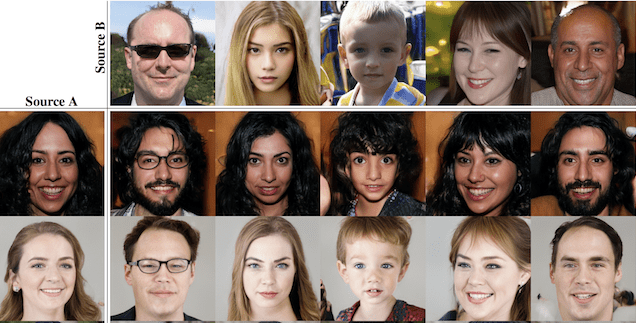
\includegraphics[scale=0.40]{images/stylegan_example1.png}
        \caption{Example of One Set of Generated Faces (Left) Adopting the Coarse Style of Another Set of Generated Faces (Top) Taken from: A Style-Based Generator Architecture for Generative Adversarial Networks.}
        }
		%\vspace*{-1mm}
	\end{figure}
	\begin{itemize}
		\item<1-> GAN: Lacking Control Over Synthesized Images
		\item<2-> Style Generative Adversarial Network(StyleGAN) Controls Style Using New Generator Model
        \item<3-> StyleGan is proficient in producing impressively photorealistic high-quality photos of faces and grants control over the characteristic of the created image at different specification levels by changing the style vectors and noise.
	\end{itemize}
        
\end{frame}

\begin{frame}
    \title{StyleGAN Model Architecture}
	\begin{figure}[h!]
		%\vspace*{-1mm}
		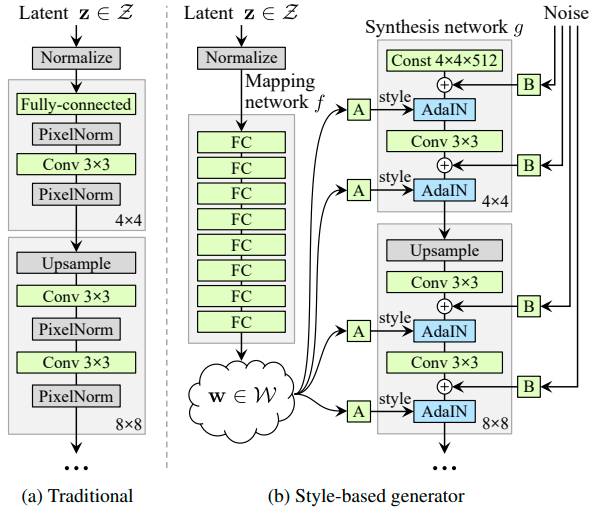
\includegraphics[scale=0.40]{images/StyleGan_Architecture.png}
		%\vspace*{-4mm}
	\end{figure}
    \textbf{The StyleGAN is described as a progressive growing GAN architecture with five modifications, each of which was added and evaluated incrementally in an ablative study.
    The incremental list of changes to the generator are:}
    \begin{itemize}
        \item Baseline Progressive GAN.
        \item Addition of tuning and bilinear upsampling.
        \item Addition of mapping network and AdaIN (styles).
        \item Removal of latent vector input to generator.
        \item Addition of noise to each block.
        \item Addition Mixing regularization.
    \end{itemize}

\end{frame}

\begin{frame}
    \title{CycleGAN}
    \textbf{Style transfer problem: change the style of an image while preserving the content.}
	\begin{figure}[h!]
		%\vspace*{-1mm}
		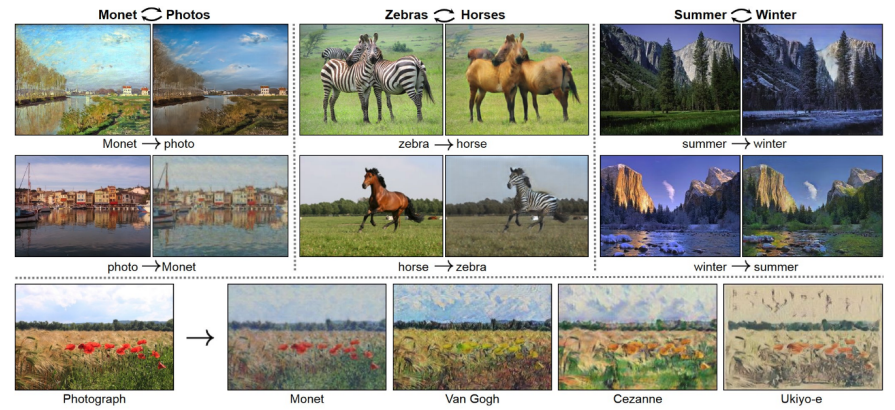
\includegraphics[scale=0.40]{images/cyclegan1.png}
		%\vspace*{-4mm}
	\end{figure}
    \textbf{Data: Two unrelated collections of images, one for each style}
\end{frame}

\begin{frame}
    \title{CycleGAN}
    \begin{itemize}
        \item If we had paired data (same content in both styles), this would be a supervised learning problem. But this is hard to find.
        \item The CycleGAN architecture learns to do it from unpaired data.
        \begin{itemize}
            \item Train two different generator nets to go from style 1 to style 2, and vice versa.
            \item Make sure the generated samples of style 2 are indistinguishable from real images by a discriminator net.
            \item Make sure the generators are cycle-consistent: mapping from style 1 to style 2 and back again should give you almost the original image.
        \end{itemize}
    \end{itemize}
\end{frame}

\begin{frame}
    \title{CycleGAN}
	\begin{figure}[h!]
		%\vspace*{-1mm}
		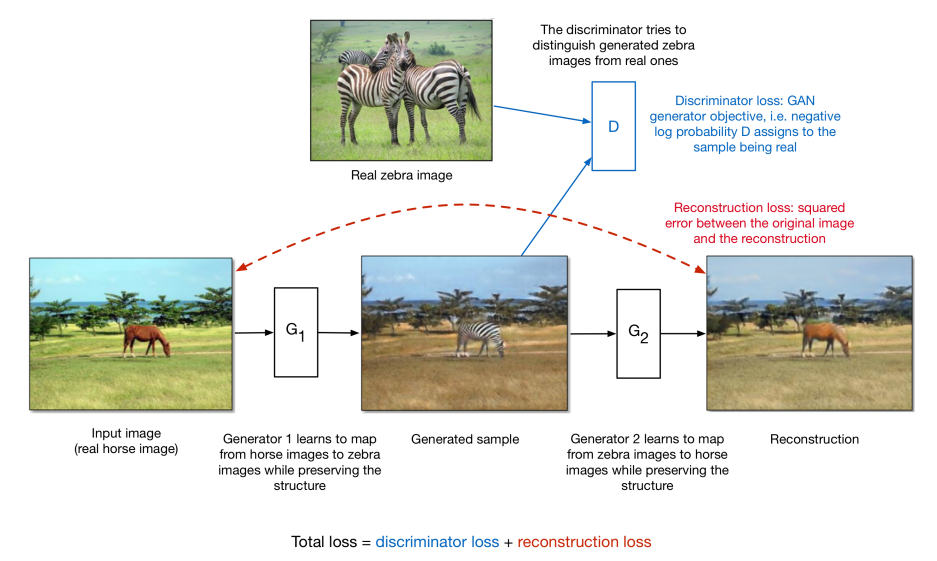
\includegraphics[scale=0.40]{images/cyclegan2.png}
		%\vspace*{-4mm}
	\end{figure}
\end{frame}

\begin{frame}
    \title{CycleGAN}
    \textbf{Style transfer between aerial photos and maps:}
	\begin{figure}[h!]
		%\vspace*{-1mm}
		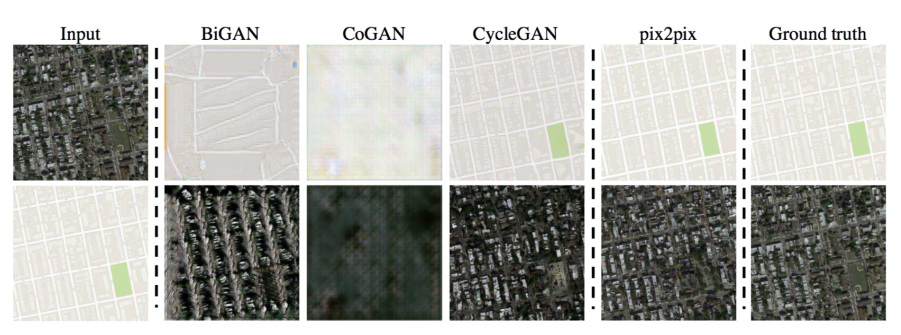
\includegraphics[scale=0.40]{images/cyclegan3.png}
		%\vspace*{-4mm}
	\end{figure}
\end{frame}

\begin{frame}
    \title{CycleGAN}
    \textbf{Style transfer between road scenes and semantic segmentations (labels of every pixel in an image by object category):}
	\begin{figure}[h!]
		%\vspace*{-1mm}
		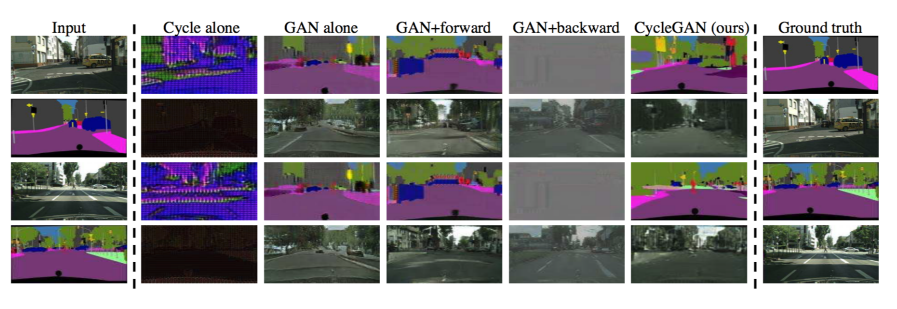
\includegraphics[scale=0.40]{images/cyclegan4.png}
		%\vspace*{-4mm}
	\end{figure}
\end{frame}

\section{StyleGAN + CycleGAN}
\begin{frame}
    \frame{\frametitle{Module 23.1: Generative Adversarial Networks - StyleGAN + CycleGAN}}

    % \myheading{Section 5: StyleGANs}
\end{frame}

\begin{frame}
    \begin{figure}[h!]
        \hyperlink{StyleGAN}{
            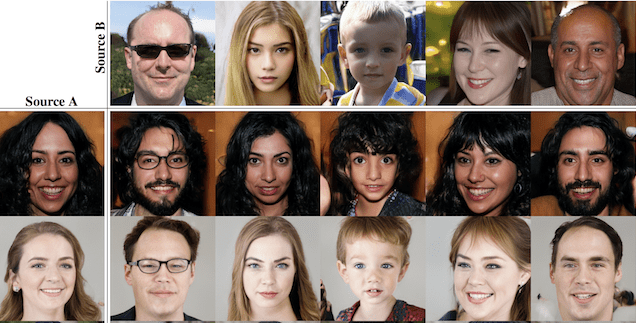
\includegraphics[scale=0.40]{images/stylegan_example1.png}
            \caption{Example of One Set of Generated Faces (Left) Adopting the Coarse Style of Another Set of Generated Faces (Top)}
        }
    \end{figure}
    \begin{itemize}
        \item GAN: Lacking Control Over Synthesized Images
        \item Style Generative Adversarial Network(StyleGAN) Controls Style Using New Generator Model
        \item StyleGan is proficient in producing impressively photorealistic high-quality photos of faces and grants control over the characteristic of the created image at different specification levels by changing the style vectors and noise.
    \end{itemize}

\end{frame}

\frame{\frametitle{StyleGAN Model Architecture}
    \hyperlink{StyleGAN}{
        \begin{figure}[h!]
            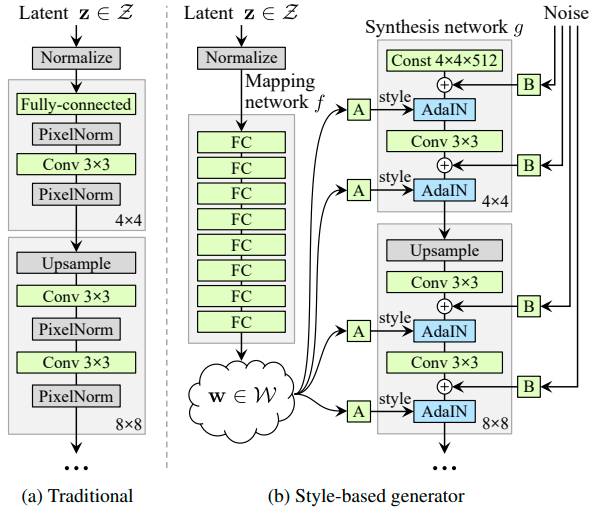
\includegraphics[width=6cm]{images/StyleGan_Architecture.png}
            \caption{StyleGAN Architecture \href{https://arxiv.org/abs/1812.04948}{(Source)}}
        \end{figure}
    }

}
\frame{\frametitle{StyleGAN Model Architecture}
    \begin{itemize}
        \item The StyleGAN is described as a progressive growing GAN architecture with five modifications:
              \begin{itemize}
                  \item Baseline Progressive GAN.
                  \item Addition of tuning and bilinear upsampling.
                  \item Addition of mapping network and AdaIN (styles).
                  \item Removal of latent vector input to generator.
                  \item Addition of noise to each block.
                  \item Addition Mixing regularization.
              \end{itemize}
    \end{itemize}
}
\begin{frame}
    \frametitle{CycleGAN: Unpaired Image-to-Image Translation}
    \begin{itemize}
        \item Style transfer problem: change the style of an image while preserving the content.
    \end{itemize}
    \hyperlink{CycleGAN}{
        \begin{figure}[h!]
            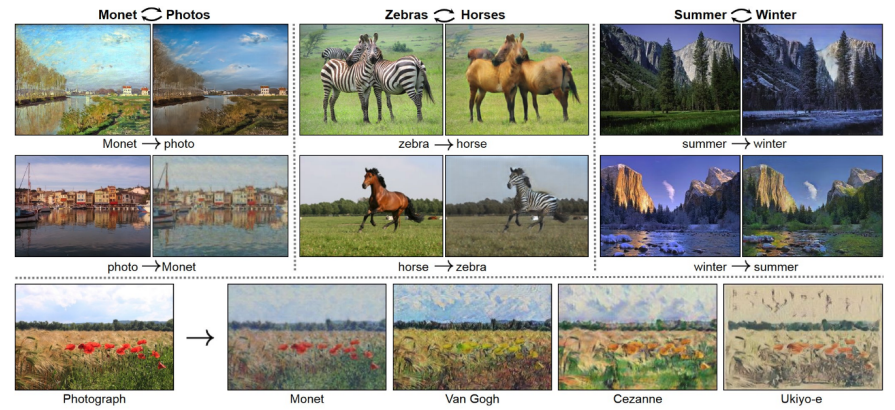
\includegraphics[scale=0.40]{images/cyclegan1.png}
        \end{figure}
    }
    \begin{itemize}
        \item Data: Two unrelated collections of images, one for each style
    \end{itemize}
\end{frame}

\begin{frame}
    \frametitle{CycleGAN: Unpaired Image-to-Image Translation}
    \begin{itemize}
        \item If we had paired data (same content in both styles), this would be a supervised learning problem. But this is hard to find.
        \item The CycleGAN architecture learns to do it from unpaired data.
              \begin{itemize}
                  \item Train two different generator nets to go from style 1 to style 2, and vice versa.
                  \item Make sure the generated samples of style 2 are indistinguishable from real images by a discriminator net.
                  \item Make sure the generators are cycle-consistent: mapping from style 1 to style 2 and back again should give you almost the original image.
              \end{itemize}
    \end{itemize}
\end{frame}

\begin{frame}
    \frametitle{CycleGAN}
    \hyperlink{CycleGAN}{
        \begin{figure}[h!]
            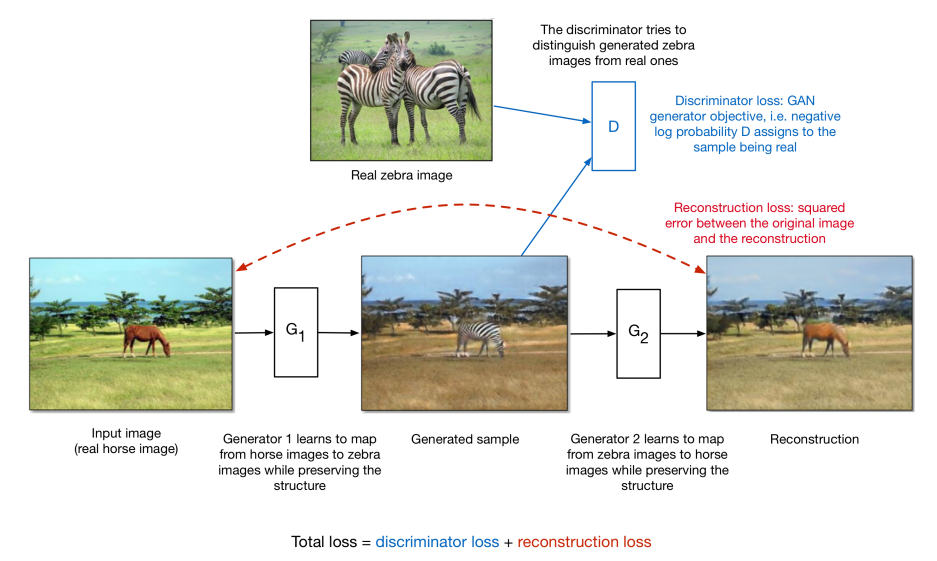
\includegraphics[scale=0.40]{images/cyclegan2.png}
        \end{figure}
    }
\end{frame}

\begin{frame}
    \frametitle{CycleGAN}
    \textbf{Style transfer between aerial photos and maps:}
    \hyperlink{CycleGAN}{
        \begin{figure}[h!]
            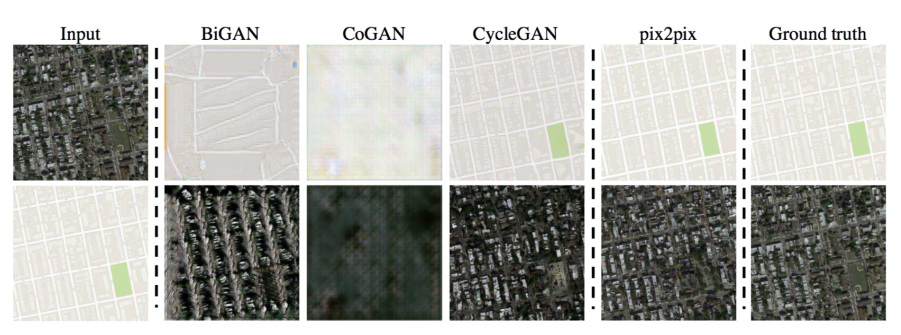
\includegraphics[scale=0.40]{images/cyclegan3.png}
        \end{figure}
    }
\end{frame}

\begin{frame}
    \frametitle{CycleGAN: Example}
    \begin{itemize}
        \item Style transfer between road scenes and semantic segmentations (labels of every pixel in an image by object category):
    \end{itemize}
    \hyperlink{CycleGAN}{
        \begin{figure}[h!]
            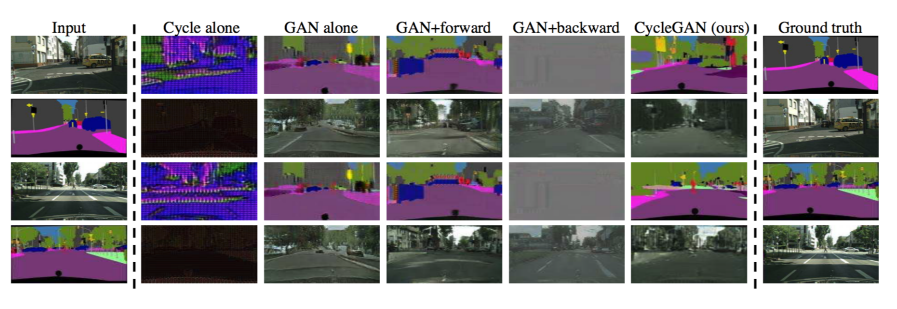
\includegraphics[scale=0.40]{images/cyclegan4.png}
        \end{figure}
    }
\end{frame}

% \section{Refrences}
\begin{frame}
    \frametitle{Image References}
    	
    \begin{itemize}
        \item \hypertarget{miteshk}{https://www.cse.iitm.ac.in/~miteshk/CS7015}
    	
    	\item \hypertarget{DCGAN}{Alec Radford, Luke Metz, Soumith Chintala Unsupervised Representation Learning with Deep Convolutional Generative Adversarial Networks(https://arxiv.org/abs/1511.06434)}
    
        \item \hypertarget{CAN}{Phillip Isola, Jun-Yan Zhu, Tinghui Zhou, Alexei A. Efros Image-to-Image Translation with Conditional Adversarial Networks(https://arxiv.org/abs/1511.06434)}
    
        \item \hypertarget{StyleGAN}{Tero Karras, Samuli Laine, Timo Aila A Style-Based Generator Architecture for Generative Adversarial Networks(https://arxiv.org/abs/1812.04948)}
    
        \item \hypertarget{CycleGAN}{Jun-Yan Zhu, Taesung Park, Phillip Isola, Alexei A. Efros Unpaired Image-to-Image Translation using Cycle-Consistent Adversarial Networks(https://arxiv.org/abs/1703.10593)}

        \item \hypertarget{GAN}{Ian Goodfellow NIPS 2016 Tutorial: Generative Adversarial Networks(https://arxiv.org/abs/1701.00160)}
        
    \end{itemize}	
\end{frame}
\section{Refrences}
\frame{
	\frametitle{Image References}
	\begin{itemize}
		\item \hypertarget{miteshk}{https://www.cse.iitm.ac.in/~miteshk/CS7015}

		\item \hypertarget{DCGAN}{Alec Radford, Luke Metz, Soumith Chintala Unsupervised Representation Learning with Deep Convolutional Generative Adversarial Networks(https://arxiv.org/abs/1511.06434)}

		\item \hypertarget{CAN}{Phillip Isola, Jun-Yan Zhu, Tinghui Zhou, Alexei A. Efros Image-to-Image Translation with Conditional Adversarial Networks(https://arxiv.org/abs/1511.06434)}

		\item \hypertarget{StyleGAN}{Tero Karras, Samuli Laine, Timo Aila A Style-Based Generator Architecture for Generative Adversarial Networks(https://arxiv.org/abs/1812.04948)}

		\item \hypertarget{CycleGAN}{Jun-Yan Zhu, Taesung Park, Phillip Isola, Alexei A. Efros Unpaired Image-to-Image Translation using Cycle-Consistent Adversarial Networks(https://arxiv.org/abs/1703.10593)}

		\item \hypertarget{GAN}{Ian Goodfellow NIPS 2016 Tutorial: Generative Adversarial Networks(https://arxiv.org/abs/1701.00160)}

		\item
		      \hypertarget{structure}{https://kdnuggets.com/2017/01/generative-adversarial-networks-hot-topic-machine-learning.html}

	\end{itemize}
}
\frame{
	\frametitle{Image References}
	\begin{itemize}

		\item
		      \hypertarget{gan}{https://www.researchgate.net/figure/Our-text-conditional-convolutional-GAN-architecture-Text-encoding-pht-is-used-by-both\_fig2\_303337197}

		\item
		      \hypertarget{why_gan}{https://www.linkedin.com/in/tauil-abd-elilah-076967176/}

		\item
		      \hypertarget{why_gan2}{https://this-person-does-not-exist.com}

		\item
		      \hypertarget{gen_disc}{https://medium.com/@jordi299/about-generative-and-discriminative-models-d8958b67ad32}


		\item
		      \hypertarget{training}{https://www.researchgate.net/figure/Overview-of-the-GAN-training-process-Segmented-volumetric-images-are-usually-split-into\_fig11\_316029770}

		\item
		      \hypertarget{GAN_paper}{Ian J. Goodfellow, Jean Pouget-Abadie, Mehdi Mirza, Bing Xu, David Warde-Farley, Sherjil Ozair, Aaron Courville, Yoshua Bengio: Generative Adversarial Networks (https://arxiv.org/abs/1406.2661)}

		\item
		      \hypertarget{applications}{
			      https://www.researchgate.net/figure/Progress-of-human-face-generation-with-GAN\_fig2\_338979046}

	\end{itemize}
}

%%%%%%%%%%%%%%%%%%%%%%%%%%%%%%%%%%%%%%%%%%
\end{document}